% Options for packages loaded elsewhere
\PassOptionsToPackage{unicode}{hyperref}
\PassOptionsToPackage{hyphens}{url}
%
\documentclass[
]{article}
\usepackage{lmodern}
\usepackage{amssymb,amsmath}
\usepackage{ifxetex,ifluatex}
\ifnum 0\ifxetex 1\fi\ifluatex 1\fi=0 % if pdftex
  \usepackage[T1]{fontenc}
  \usepackage[utf8]{inputenc}
  \usepackage{textcomp} % provide euro and other symbols
\else % if luatex or xetex
  \usepackage{unicode-math}
  \defaultfontfeatures{Scale=MatchLowercase}
  \defaultfontfeatures[\rmfamily]{Ligatures=TeX,Scale=1}
\fi
% Use upquote if available, for straight quotes in verbatim environments
\IfFileExists{upquote.sty}{\usepackage{upquote}}{}
\IfFileExists{microtype.sty}{% use microtype if available
  \usepackage[]{microtype}
  \UseMicrotypeSet[protrusion]{basicmath} % disable protrusion for tt fonts
}{}
\makeatletter
\@ifundefined{KOMAClassName}{% if non-KOMA class
  \IfFileExists{parskip.sty}{%
    \usepackage{parskip}
  }{% else
    \setlength{\parindent}{0pt}
    \setlength{\parskip}{6pt plus 2pt minus 1pt}}
}{% if KOMA class
  \KOMAoptions{parskip=half}}
\makeatother
\usepackage{xcolor}
\IfFileExists{xurl.sty}{\usepackage{xurl}}{} % add URL line breaks if available
\IfFileExists{bookmark.sty}{\usepackage{bookmark}}{\usepackage{hyperref}}
\hypersetup{
  pdftitle={Data-analysis},
  hidelinks,
  pdfcreator={LaTeX via pandoc}}
\urlstyle{same} % disable monospaced font for URLs
\usepackage[margin=1in]{geometry}
\usepackage{color}
\usepackage{fancyvrb}
\newcommand{\VerbBar}{|}
\newcommand{\VERB}{\Verb[commandchars=\\\{\}]}
\DefineVerbatimEnvironment{Highlighting}{Verbatim}{commandchars=\\\{\}}
% Add ',fontsize=\small' for more characters per line
\usepackage{framed}
\definecolor{shadecolor}{RGB}{248,248,248}
\newenvironment{Shaded}{\begin{snugshade}}{\end{snugshade}}
\newcommand{\AlertTok}[1]{\textcolor[rgb]{0.94,0.16,0.16}{#1}}
\newcommand{\AnnotationTok}[1]{\textcolor[rgb]{0.56,0.35,0.01}{\textbf{\textit{#1}}}}
\newcommand{\AttributeTok}[1]{\textcolor[rgb]{0.77,0.63,0.00}{#1}}
\newcommand{\BaseNTok}[1]{\textcolor[rgb]{0.00,0.00,0.81}{#1}}
\newcommand{\BuiltInTok}[1]{#1}
\newcommand{\CharTok}[1]{\textcolor[rgb]{0.31,0.60,0.02}{#1}}
\newcommand{\CommentTok}[1]{\textcolor[rgb]{0.56,0.35,0.01}{\textit{#1}}}
\newcommand{\CommentVarTok}[1]{\textcolor[rgb]{0.56,0.35,0.01}{\textbf{\textit{#1}}}}
\newcommand{\ConstantTok}[1]{\textcolor[rgb]{0.00,0.00,0.00}{#1}}
\newcommand{\ControlFlowTok}[1]{\textcolor[rgb]{0.13,0.29,0.53}{\textbf{#1}}}
\newcommand{\DataTypeTok}[1]{\textcolor[rgb]{0.13,0.29,0.53}{#1}}
\newcommand{\DecValTok}[1]{\textcolor[rgb]{0.00,0.00,0.81}{#1}}
\newcommand{\DocumentationTok}[1]{\textcolor[rgb]{0.56,0.35,0.01}{\textbf{\textit{#1}}}}
\newcommand{\ErrorTok}[1]{\textcolor[rgb]{0.64,0.00,0.00}{\textbf{#1}}}
\newcommand{\ExtensionTok}[1]{#1}
\newcommand{\FloatTok}[1]{\textcolor[rgb]{0.00,0.00,0.81}{#1}}
\newcommand{\FunctionTok}[1]{\textcolor[rgb]{0.00,0.00,0.00}{#1}}
\newcommand{\ImportTok}[1]{#1}
\newcommand{\InformationTok}[1]{\textcolor[rgb]{0.56,0.35,0.01}{\textbf{\textit{#1}}}}
\newcommand{\KeywordTok}[1]{\textcolor[rgb]{0.13,0.29,0.53}{\textbf{#1}}}
\newcommand{\NormalTok}[1]{#1}
\newcommand{\OperatorTok}[1]{\textcolor[rgb]{0.81,0.36,0.00}{\textbf{#1}}}
\newcommand{\OtherTok}[1]{\textcolor[rgb]{0.56,0.35,0.01}{#1}}
\newcommand{\PreprocessorTok}[1]{\textcolor[rgb]{0.56,0.35,0.01}{\textit{#1}}}
\newcommand{\RegionMarkerTok}[1]{#1}
\newcommand{\SpecialCharTok}[1]{\textcolor[rgb]{0.00,0.00,0.00}{#1}}
\newcommand{\SpecialStringTok}[1]{\textcolor[rgb]{0.31,0.60,0.02}{#1}}
\newcommand{\StringTok}[1]{\textcolor[rgb]{0.31,0.60,0.02}{#1}}
\newcommand{\VariableTok}[1]{\textcolor[rgb]{0.00,0.00,0.00}{#1}}
\newcommand{\VerbatimStringTok}[1]{\textcolor[rgb]{0.31,0.60,0.02}{#1}}
\newcommand{\WarningTok}[1]{\textcolor[rgb]{0.56,0.35,0.01}{\textbf{\textit{#1}}}}
\usepackage{graphicx,grffile}
\makeatletter
\def\maxwidth{\ifdim\Gin@nat@width>\linewidth\linewidth\else\Gin@nat@width\fi}
\def\maxheight{\ifdim\Gin@nat@height>\textheight\textheight\else\Gin@nat@height\fi}
\makeatother
% Scale images if necessary, so that they will not overflow the page
% margins by default, and it is still possible to overwrite the defaults
% using explicit options in \includegraphics[width, height, ...]{}
\setkeys{Gin}{width=\maxwidth,height=\maxheight,keepaspectratio}
% Set default figure placement to htbp
\makeatletter
\def\fps@figure{htbp}
\makeatother
\setlength{\emergencystretch}{3em} % prevent overfull lines
\providecommand{\tightlist}{%
  \setlength{\itemsep}{0pt}\setlength{\parskip}{0pt}}
\setcounter{secnumdepth}{-\maxdimen} % remove section numbering

\title{Data-analysis}
\author{}
\date{\vspace{-2.5em}}

\begin{document}
\maketitle

\begin{Shaded}
\begin{Highlighting}[]
\KeywordTok{library}\NormalTok{(tidyverse)}
\KeywordTok{library}\NormalTok{(lubridate)}
\KeywordTok{library}\NormalTok{(readr)}
\KeywordTok{library}\NormalTok{(janitor)}
\KeywordTok{library}\NormalTok{(patchwork)}
\KeywordTok{library}\NormalTok{(scales)}
\KeywordTok{library}\NormalTok{(moderndive)}
\KeywordTok{library}\NormalTok{(stats)}
\KeywordTok{library}\NormalTok{(skimr)}
\KeywordTok{library}\NormalTok{(kableExtra)}
\end{Highlighting}
\end{Shaded}

For this project we are using two datasets available from the CDC.

The first is a dataset that includes weekly estimates of expected deaths
by week for each US states, as well as observed deaths. It is available
for download here:
\url{https://data.cdc.gov/NCHS/Excess-Deaths-Associated-with-COVID-19/xkkf-xrst/}

\begin{Shaded}
\begin{Highlighting}[]
\NormalTok{excess_deaths <-}\StringTok{ }\KeywordTok{read_csv}\NormalTok{(}\StringTok{"data/Excess_Deaths_Associated_with_COVID-19.csv"}\NormalTok{) }\OperatorTok\StringTok{ }
\StringTok{  }\KeywordTok{clean_names}\NormalTok{() }\OperatorTok\StringTok{ }
\StringTok{  }\KeywordTok{rename}\NormalTok{(}\DataTypeTok{end_week=}\NormalTok{week_ending_date) }\OperatorTok\StringTok{ }
\StringTok{  }\KeywordTok{filter}\NormalTok{(type}\OperatorTok{==}\StringTok{"Predicted (weighted)"}\OperatorTok{&}\NormalTok{outcome}\OperatorTok{==}\StringTok{"All causes"}\NormalTok{) }
\end{Highlighting}
\end{Shaded}

The second dataset includes the weekly counts of COVID-19 related deaths
in each US state. And is available here:
\url{https://data.cdc.gov/NCHS/Provisional-COVID-19-Death-Counts-by-Week-Ending-D/r8kw-7aab}

\begin{Shaded}
\begin{Highlighting}[]
\NormalTok{covid_deaths <-}\StringTok{ }\KeywordTok{read_csv}\NormalTok{(}\StringTok{"data/Provisional_COVID-19_Death_Counts_by_Week_Ending_Date_and_State.csv"}\NormalTok{) }\OperatorTok\StringTok{ }
\StringTok{  }\KeywordTok{clean_names}\NormalTok{() }\OperatorTok
\StringTok{  }\KeywordTok{mutate}\NormalTok{(}\DataTypeTok{end_week=}\KeywordTok{mdy}\NormalTok{(end_week))}\OperatorTok
\StringTok{  }\KeywordTok{select}\NormalTok{(end_week,state,covid_}\DecValTok{19}\NormalTok{_deaths,total_deaths,percent_of_expected_deaths,pneumonia_deaths, pneumonia_and_covid_}\DecValTok{19}\NormalTok{_deaths, influenza_deaths, pneumonia_influenza_or_covid_}\DecValTok{19}\NormalTok{_deaths) }

\NormalTok{merged_data <-}\StringTok{ }\KeywordTok{inner_join}\NormalTok{(covid_deaths,excess_deaths) }\OperatorTok\StringTok{ }
\StringTok{  }\KeywordTok{mutate}\NormalTok{(}\DataTypeTok{excess_non_covid=}\NormalTok{excess_higher_estimate}\OperatorTok{-}\NormalTok{covid_}\DecValTok{19}\NormalTok{_deaths)}
\end{Highlighting}
\end{Shaded}

These datasets are updated frequently. This analysis is based on data
downloaded on December 1, 2020. Also because death reporting takes time
this analysis focuses on deaths reported through the end of October
2020.

To explore the relationship between excess deaths, deaths attributed to
COVID-19, and excess deaths that were not attributed to COVID-19, we
generated time series plots for these quantities for the entire nation.

\begin{Shaded}
\begin{Highlighting}[]
\NormalTok{panel1=merged_data }\OperatorTok\StringTok{ }
\StringTok{  }\KeywordTok{filter}\NormalTok{(state}\OperatorTok{==}\StringTok{"United States"}\NormalTok{) }\OperatorTok\StringTok{ }
\StringTok{   }\KeywordTok{ggplot}\NormalTok{(}\KeywordTok{aes}\NormalTok{(}\DataTypeTok{x=}\NormalTok{end_week,}\DataTypeTok{y=}\NormalTok{covid_}\DecValTok{19}\NormalTok{_deaths))}\OperatorTok{+}
\StringTok{   }\KeywordTok{labs}\NormalTok{(}\DataTypeTok{x =} \StringTok{"Date"}\NormalTok{, }\DataTypeTok{y =} \StringTok{"COVID-19 deaths"}\NormalTok{) }\OperatorTok{+}
\StringTok{   }\KeywordTok{geom_point}\NormalTok{(}\DataTypeTok{alpha=}\FloatTok{0.5}\NormalTok{, }\DataTypeTok{size=}\DecValTok{3}\NormalTok{)}\OperatorTok{+}
\StringTok{   }\KeywordTok{geom_smooth}\NormalTok{(}\DataTypeTok{se=}\OtherTok{FALSE}\NormalTok{, }\DataTypeTok{span=}\FloatTok{0.2}\NormalTok{) }\OperatorTok{+}
\StringTok{    }\KeywordTok{scale_x_date}\NormalTok{(}
    \DataTypeTok{labels =} \KeywordTok{date_format}\NormalTok{(}\StringTok{"%m-%Y"}\NormalTok{),}
    \DataTypeTok{breaks=} \KeywordTok{c}\NormalTok{(}\KeywordTok{as.Date}\NormalTok{(}\StringTok{"2020/2/1"}\NormalTok{),}\KeywordTok{as.Date}\NormalTok{(}\StringTok{"2020/5/1"}\NormalTok{),}\KeywordTok{as.Date}\NormalTok{(}\StringTok{"2020/8/1"}\NormalTok{), }\KeywordTok{as.Date}\NormalTok{(}\StringTok{"2020/11/1"}\NormalTok{)),}
    \DataTypeTok{limits=} \KeywordTok{c}\NormalTok{(}\KeywordTok{as.Date}\NormalTok{(}\StringTok{"2020/2/1"}\NormalTok{), }\KeywordTok{as.Date}\NormalTok{(}\StringTok{"2020/10/31"}\NormalTok{)))}\OperatorTok{+}
\StringTok{  }\KeywordTok{theme}\NormalTok{(}\DataTypeTok{axis.text.x=}\KeywordTok{element_text}\NormalTok{(}\DataTypeTok{angle=}\DecValTok{45}\NormalTok{,}\DataTypeTok{hjust=}\DecValTok{1}\NormalTok{))}\OperatorTok{+}
\StringTok{   }\KeywordTok{scale_y_continuous}\NormalTok{(}\DataTypeTok{limits=}\KeywordTok{c}\NormalTok{(}\OperatorTok{-}\DecValTok{1000}\NormalTok{, }\DecValTok{25000}\NormalTok{))}


\NormalTok{panel2=}\StringTok{ }\NormalTok{merged_data  }\OperatorTok\StringTok{ }
\StringTok{  }\KeywordTok{filter}\NormalTok{(state}\OperatorTok{==}\StringTok{"United States"}\NormalTok{) }\OperatorTok\StringTok{ }
\StringTok{   }\KeywordTok{ggplot}\NormalTok{(}\KeywordTok{aes}\NormalTok{(}\DataTypeTok{x=}\NormalTok{end_week,}\DataTypeTok{y=}\NormalTok{excess_higher_estimate))}\OperatorTok{+}
\StringTok{   }\KeywordTok{labs}\NormalTok{(}\DataTypeTok{x =} \StringTok{"Date"}\NormalTok{, }\DataTypeTok{y =} \StringTok{"Excess deaths"}\NormalTok{) }\OperatorTok{+}
\StringTok{   }\KeywordTok{geom_point}\NormalTok{(}\DataTypeTok{alpha=}\FloatTok{0.5}\NormalTok{, }\DataTypeTok{size=}\DecValTok{3}\NormalTok{)}\OperatorTok{+}
\StringTok{   }\KeywordTok{geom_smooth}\NormalTok{(}\DataTypeTok{se=}\OtherTok{FALSE}\NormalTok{, }\DataTypeTok{span=}\FloatTok{0.2}\NormalTok{) }\OperatorTok{+}
\StringTok{    }\KeywordTok{scale_x_date}\NormalTok{(}
    \DataTypeTok{labels =} \KeywordTok{date_format}\NormalTok{(}\StringTok{"%m-%Y"}\NormalTok{),}
    \DataTypeTok{breaks=} \KeywordTok{c}\NormalTok{(}\KeywordTok{as.Date}\NormalTok{(}\StringTok{"2020/2/1"}\NormalTok{),}\KeywordTok{as.Date}\NormalTok{(}\StringTok{"2020/5/1"}\NormalTok{),}\KeywordTok{as.Date}\NormalTok{(}\StringTok{"2020/8/1"}\NormalTok{), }\KeywordTok{as.Date}\NormalTok{(}\StringTok{"2020/11/1"}\NormalTok{)),}
    \DataTypeTok{limits=} \KeywordTok{c}\NormalTok{(}\KeywordTok{as.Date}\NormalTok{(}\StringTok{"2020/2/1"}\NormalTok{), }\KeywordTok{as.Date}\NormalTok{(}\StringTok{"2020/10/31"}\NormalTok{)))}\OperatorTok{+}
\StringTok{  }\KeywordTok{theme}\NormalTok{(}\DataTypeTok{axis.text.x=}\KeywordTok{element_text}\NormalTok{(}\DataTypeTok{angle=}\DecValTok{45}\NormalTok{,}\DataTypeTok{hjust=}\DecValTok{1}\NormalTok{))}\OperatorTok{+}
\StringTok{   }\KeywordTok{scale_y_continuous}\NormalTok{(}\DataTypeTok{limits=}\KeywordTok{c}\NormalTok{(}\OperatorTok{-}\DecValTok{1000}\NormalTok{, }\DecValTok{25000}\NormalTok{))}

\NormalTok{panel3=}
\StringTok{ }\NormalTok{merged_data }\OperatorTok
\StringTok{  }\KeywordTok{filter}\NormalTok{(state}\OperatorTok{==}\StringTok{"United States"}\NormalTok{) }\OperatorTok\StringTok{ }
\StringTok{  }\KeywordTok{ggplot}\NormalTok{(}\KeywordTok{aes}\NormalTok{(}\DataTypeTok{x=}\NormalTok{end_week,}\DataTypeTok{y=}\NormalTok{excess_non_covid))}\OperatorTok{+}
\StringTok{   }\KeywordTok{labs}\NormalTok{(}\DataTypeTok{x =} \StringTok{"Date"}\NormalTok{, }\DataTypeTok{y =} \StringTok{"Excess deaths not attributed to COVID-19"}\NormalTok{) }\OperatorTok{+}
\StringTok{   }\KeywordTok{geom_point}\NormalTok{(}\DataTypeTok{alpha=}\FloatTok{0.5}\NormalTok{, }\DataTypeTok{size=}\DecValTok{3}\NormalTok{)}\OperatorTok{+}
\StringTok{   }\KeywordTok{geom_smooth}\NormalTok{(}\DataTypeTok{se=}\OtherTok{FALSE}\NormalTok{, }\DataTypeTok{span=}\FloatTok{0.2}\NormalTok{) }\OperatorTok{+}
\StringTok{    }\KeywordTok{scale_x_date}\NormalTok{(}
    \DataTypeTok{labels =} \KeywordTok{date_format}\NormalTok{(}\StringTok{"%m-%Y"}\NormalTok{),}
    \DataTypeTok{breaks=} \KeywordTok{c}\NormalTok{(}\KeywordTok{as.Date}\NormalTok{(}\StringTok{"2020/2/1"}\NormalTok{),}\KeywordTok{as.Date}\NormalTok{(}\StringTok{"2020/5/1"}\NormalTok{),}\KeywordTok{as.Date}\NormalTok{(}\StringTok{"2020/8/1"}\NormalTok{), }\KeywordTok{as.Date}\NormalTok{(}\StringTok{"2020/11/1"}\NormalTok{)),}
    \DataTypeTok{limits=} \KeywordTok{c}\NormalTok{(}\KeywordTok{as.Date}\NormalTok{(}\StringTok{"2020/2/1"}\NormalTok{), }\KeywordTok{as.Date}\NormalTok{(}\StringTok{"2020/10/31"}\NormalTok{)))}\OperatorTok{+}
\StringTok{  }\KeywordTok{theme}\NormalTok{(}\DataTypeTok{axis.text.x=}\KeywordTok{element_text}\NormalTok{(}\DataTypeTok{angle=}\DecValTok{45}\NormalTok{,}\DataTypeTok{hjust=}\DecValTok{1}\NormalTok{))}\OperatorTok{+}
\StringTok{   }\KeywordTok{scale_y_continuous}\NormalTok{(}\DataTypeTok{limits=}\KeywordTok{c}\NormalTok{(}\OperatorTok{-}\DecValTok{1000}\NormalTok{, }\DecValTok{25000}\NormalTok{))}

\NormalTok{panel2 }\OperatorTok{+}\StringTok{ }\NormalTok{panel1 }\OperatorTok{+}\StringTok{ }\NormalTok{panel3}
\end{Highlighting}
\end{Shaded}

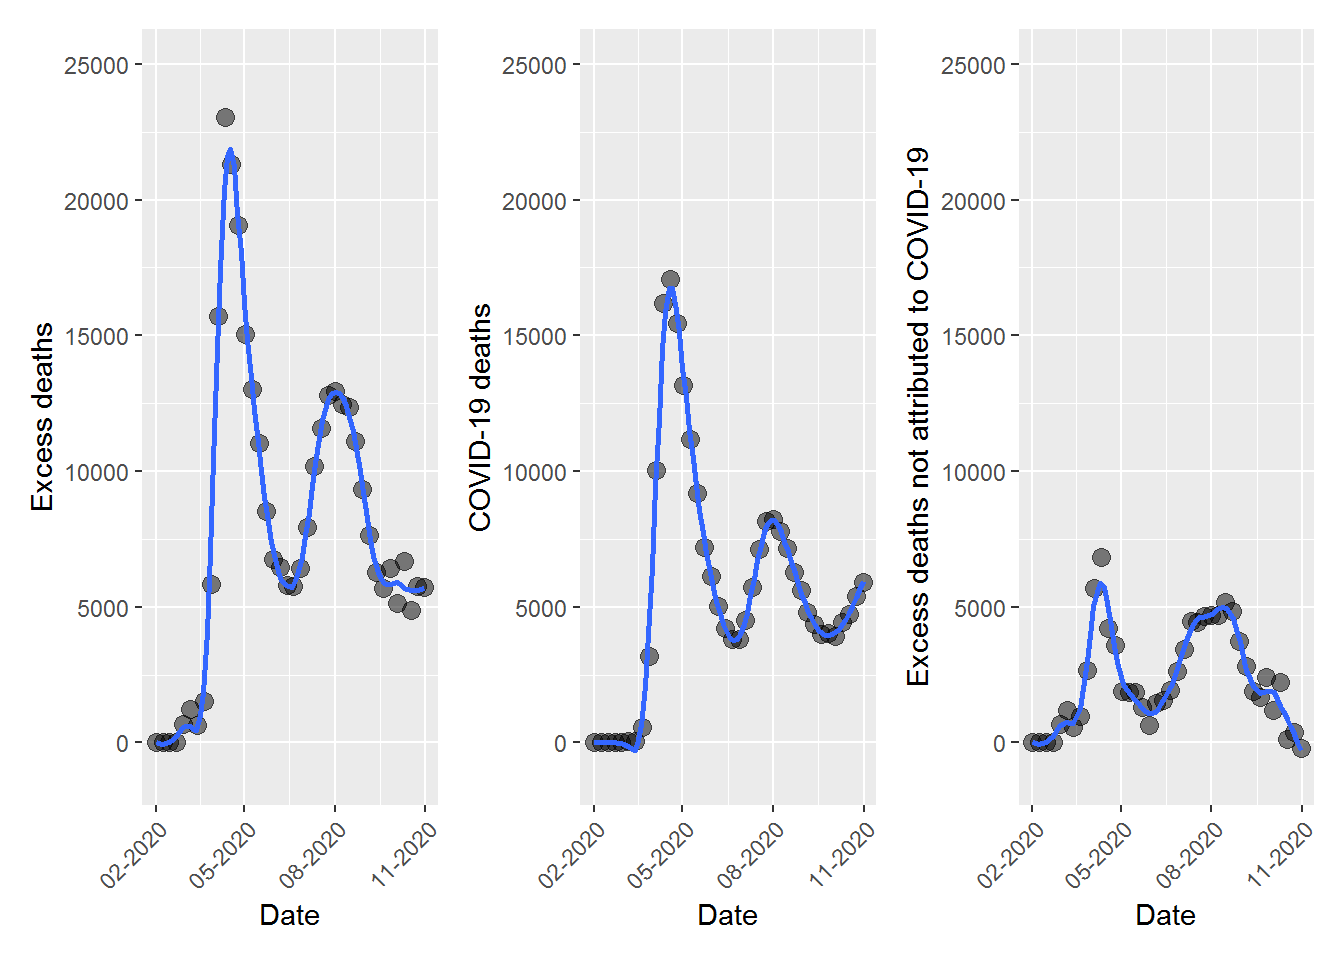
\includegraphics{analysis_files/figure-latex/unnamed-chunk-4-1.pdf} This
code chunk calculates the number of excess deaths, covid deaths, and
excess non-covid deaths in the United States from February through
October 2020.

\begin{Shaded}
\begin{Highlighting}[]
\NormalTok{merged_data }\OperatorTok\StringTok{ }
\StringTok{  }\KeywordTok{filter}\NormalTok{(state}\OperatorTok{==}\StringTok{"United States"} \OperatorTok{&}\StringTok{ }\NormalTok{end_week }\OperatorTok{<}\StringTok{ }\KeywordTok{as.Date}\NormalTok{(}\StringTok{"2020-11-1"}\NormalTok{)) }\OperatorTok\StringTok{ }
\StringTok{  }\KeywordTok{summarise}\NormalTok{(}
    \DataTypeTok{excess_deaths=}\KeywordTok{sum}\NormalTok{(excess_higher_estimate),}
    \DataTypeTok{covid_deaths=}\KeywordTok{sum}\NormalTok{(covid_}\DecValTok{19}\NormalTok{_deaths),}
    \DataTypeTok{excess_not_covid=}\KeywordTok{sum}\NormalTok{(excess_higher_estimate)}\OperatorTok{-}\KeywordTok{sum}\NormalTok{(covid_}\DecValTok{19}\NormalTok{_deaths)) }\OperatorTok\StringTok{ }
\StringTok{   }\KeywordTok{kbl}\NormalTok{(}\DataTypeTok{caption=}\StringTok{"Excess and Covid Deaths in the United States: Feb-October, 2020"}\NormalTok{, }\DataTypeTok{digits =} \DecValTok{1}\NormalTok{) }\OperatorTok\StringTok{ }\KeywordTok{kable_classic}\NormalTok{()}
\end{Highlighting}
\end{Shaded}

\begin{table}

\caption{\label{tab:unnamed-chunk-5}Excess and Covid Deaths in the United States: Feb-October, 2020}
\centering
\begin{tabular}[t]{r|r|r}
\hline
excess\_deaths & covid\_deaths & excess\_not\_covid\\
\hline
322742 & 228524 & 94218\\
\hline
\end{tabular}
\end{table}

Approximately 1/3 of excess deaths were not attributed to COVID.

Next I was interested in getting a sense of whether the rate of excess
non-COVID-19 deaths varied across States.

In the next code chunk I aggregate the data by state over the entire
period, merge the data with another data set containing state level
population estimates for 2020. I then calculate rates of COVID-19
deaths, excess deaths, and excess deaths not attributable to COVID-19
(per 100,000 residents) for each state, and calculate the median and
intraquartile range for these quatities.

\begin{Shaded}
\begin{Highlighting}[]
\NormalTok{states=}\StringTok{ }\NormalTok{merged_data }\OperatorTok\StringTok{ }
\StringTok{  }\KeywordTok{group_by}\NormalTok{(state) }\OperatorTok\StringTok{ }
\StringTok{  }\KeywordTok{filter}\NormalTok{(end_week }\OperatorTok{<}\StringTok{ }\KeywordTok{as.Date}\NormalTok{(}\StringTok{"2020-11-1"}\NormalTok{) }\OperatorTok{&}\StringTok{ }\NormalTok{state }\OperatorTok{!=}\StringTok{"United States"} \OperatorTok{&}\StringTok{ }\NormalTok{state}\OperatorTok{!=}\StringTok{"New York City"}\NormalTok{) }\OperatorTok\StringTok{ }
\StringTok{  }\KeywordTok{filter}\NormalTok{(}\OperatorTok{!}\KeywordTok{is.na}\NormalTok{(covid_}\DecValTok{19}\NormalTok{_deaths)) }\OperatorTok\StringTok{ }
\StringTok{  }\KeywordTok{filter}\NormalTok{(}\OperatorTok{!}\KeywordTok{is.na}\NormalTok{(excess_higher_estimate)) }\OperatorTok\StringTok{ }
\StringTok{  }\KeywordTok{summarise}\NormalTok{(}
    \DataTypeTok{excess_deaths=}\KeywordTok{sum}\NormalTok{(excess_higher_estimate),}
    \DataTypeTok{covid_deaths=}\KeywordTok{sum}\NormalTok{(covid_}\DecValTok{19}\NormalTok{_deaths),}
    \DataTypeTok{excess_not_covid=}\KeywordTok{sum}\NormalTok{(excess_higher_estimate)}\OperatorTok{-}\KeywordTok{sum}\NormalTok{(covid_}\DecValTok{19}\NormalTok{_deaths)) }
\end{Highlighting}
\end{Shaded}

\begin{verbatim}
## `summarise()` ungrouping output (override with `.groups` argument)
\end{verbatim}

\begin{Shaded}
\begin{Highlighting}[]
\NormalTok{state_pop <-}\StringTok{ }\KeywordTok{read_csv}\NormalTok{(}\StringTok{"data/State_Populations.csv"}\NormalTok{) }\OperatorTok\StringTok{ }
\StringTok{  }\KeywordTok{clean_names}\NormalTok{()}
\end{Highlighting}
\end{Shaded}

\begin{verbatim}
## 
## -- Column specification --------------------------------------------------------
## cols(
##   State = col_character(),
##   Population = col_double()
## )
\end{verbatim}

\begin{Shaded}
\begin{Highlighting}[]
\NormalTok{states=}\KeywordTok{right_join}\NormalTok{(states,state_pop) }\OperatorTok\StringTok{ }
\StringTok{  }\KeywordTok{mutate}\NormalTok{(}\DataTypeTok{excess_death_r=}\NormalTok{excess_deaths}\OperatorTok{/}\NormalTok{population}\OperatorTok{*}\DecValTok{100000}\NormalTok{) }\OperatorTok\StringTok{ }
\StringTok{  }\KeywordTok{mutate}\NormalTok{(}\DataTypeTok{covid_death_r=}\NormalTok{covid_deaths}\OperatorTok{/}\NormalTok{population}\OperatorTok{*}\DecValTok{100000}\NormalTok{) }\OperatorTok\StringTok{ }
\StringTok{  }\KeywordTok{mutate}\NormalTok{(}\DataTypeTok{excess_not_covid_r=}\NormalTok{excess_not_covid}\OperatorTok{/}\NormalTok{population}\OperatorTok{*}\DecValTok{100000}\NormalTok{)}
\end{Highlighting}
\end{Shaded}

\begin{verbatim}
## Joining, by = "state"
\end{verbatim}

\begin{Shaded}
\begin{Highlighting}[]
\NormalTok{states }\OperatorTok\StringTok{ }
\StringTok{  }\KeywordTok{select}\NormalTok{(excess_death_r, covid_death_r, excess_not_covid_r) }\OperatorTok\StringTok{ }
\StringTok{  }\KeywordTok{rename}\NormalTok{(}\DataTypeTok{excess_death_rate=}\NormalTok{excess_death_r,}\DataTypeTok{covid_death_rate=}\NormalTok{covid_death_r,}\DataTypeTok{excess_deaths_not_from_covid_rate=}\NormalTok{excess_not_covid_r) }\OperatorTok\StringTok{ }
\StringTok{  }\KeywordTok{skim_without_charts}\NormalTok{() }\OperatorTok\StringTok{ }
\StringTok{  }\KeywordTok{select}\NormalTok{(skim_variable, numeric.p50, numeric.p25, numeric.p75) }\OperatorTok\StringTok{ }
\StringTok{  }\KeywordTok{rename}\NormalTok{(}\DataTypeTok{Rate=}\NormalTok{skim_variable, }\DataTypeTok{Median=}\NormalTok{numeric.p50, }\DataTypeTok{p25=}\NormalTok{numeric.p25, }\DataTypeTok{p75th=}\NormalTok{numeric.p75) }\OperatorTok\StringTok{ }
\StringTok{   }\KeywordTok{kbl}\NormalTok{(}\DataTypeTok{caption=}\StringTok{"Rates of excess and COVID-19 deaths (per 100,000 residents) among US States and District of Columbia: Feb-October, 2020"}\NormalTok{, }\DataTypeTok{digits =} \DecValTok{1}\NormalTok{) }\OperatorTok\StringTok{ }
\StringTok{  }\KeywordTok{kable_classic}\NormalTok{() }
\end{Highlighting}
\end{Shaded}

\begin{table}

\caption{\label{tab:unnamed-chunk-6}Rates of excess and COVID-19 deaths (per 100,000 residents) among US States and District of Columbia: Feb-October, 2020}
\centering
\begin{tabular}[t]{l|r|r|r}
\hline
Rate & Median & p25 & p75th\\
\hline
excess\_death\_rate & 82.1 & 65.5 & 108.0\\
\hline
covid\_death\_rate & 52.3 & 39.0 & 70.5\\
\hline
excess\_deaths\_not\_from\_covid\_rate & 27.7 & 19.7 & 40.9\\
\hline
\end{tabular}
\end{table}

This state-level dataset is used to visually explore the relationships
between state-level COVID-19 death rates, excess mortality rates, and
rates of excess non-COVID-19 mortality per 100,000 residents.

\begin{Shaded}
\begin{Highlighting}[]
\NormalTok{panel4 =}\StringTok{ }\NormalTok{states }\OperatorTok\StringTok{ }
\StringTok{ }\KeywordTok{ggplot}\NormalTok{( }\KeywordTok{aes}\NormalTok{(}\DataTypeTok{x=}\NormalTok{covid_death_r,}\DataTypeTok{y=}\NormalTok{excess_not_covid_r, }\DataTypeTok{size=}\NormalTok{population))}\OperatorTok{+}
\StringTok{   }\KeywordTok{labs}\NormalTok{(}\DataTypeTok{x =} \StringTok{"COVID-19 deaths }\CharTok{\textbackslash{}n}\StringTok{ per 100,000 residents"}\NormalTok{, }\DataTypeTok{y =} \StringTok{"Excess COVID-19 deaths not attributed}\CharTok{\textbackslash{}n}\StringTok{ to COVID-19 per 100,000 residents"}\NormalTok{) }\OperatorTok{+}
\StringTok{   }\KeywordTok{geom_point}\NormalTok{(}\DataTypeTok{alpha=}\FloatTok{0.5}\NormalTok{)}\OperatorTok{+}
\StringTok{  }\KeywordTok{geom_smooth}\NormalTok{(}\DataTypeTok{weight=}\StringTok{"population"}\NormalTok{)}\OperatorTok{+}
\StringTok{  }\KeywordTok{theme}\NormalTok{(}\DataTypeTok{legend.position =} \StringTok{"none"}\NormalTok{) }\OperatorTok{+}
\StringTok{  }\KeywordTok{scale_y_continuous}\NormalTok{(}\DataTypeTok{limits=}\KeywordTok{c}\NormalTok{(}\DecValTok{0}\NormalTok{, }\DecValTok{300}\NormalTok{))}


\NormalTok{panel5 =}\StringTok{ }\NormalTok{states }\OperatorTok\StringTok{ }
\StringTok{ }\KeywordTok{ggplot}\NormalTok{( }\KeywordTok{aes}\NormalTok{(}\DataTypeTok{x=}\NormalTok{covid_death_r,}\DataTypeTok{y=}\NormalTok{excess_death_r, }\DataTypeTok{size=}\NormalTok{population))}\OperatorTok{+}
\StringTok{   }\KeywordTok{labs}\NormalTok{(}\DataTypeTok{x =} \StringTok{"COVID-19 deaths }\CharTok{\textbackslash{}n}\StringTok{ per 100,000 residents"}\NormalTok{, }\DataTypeTok{y =} \StringTok{"Excess deaths }\CharTok{\textbackslash{}n}\StringTok{ per 100,000 residents"}\NormalTok{) }\OperatorTok{+}
\StringTok{   }\KeywordTok{geom_point}\NormalTok{(}\DataTypeTok{alpha=}\FloatTok{0.5}\NormalTok{)}\OperatorTok{+}
\StringTok{  }\KeywordTok{geom_smooth}\NormalTok{(, }\DataTypeTok{weight=}\StringTok{"population"}\NormalTok{)}\OperatorTok{+}
\StringTok{ }\KeywordTok{theme}\NormalTok{(}\DataTypeTok{legend.position =} \StringTok{"none"}\NormalTok{) }\OperatorTok{+}
\StringTok{  }\KeywordTok{scale_y_continuous}\NormalTok{(}\DataTypeTok{limits=}\KeywordTok{c}\NormalTok{(}\DecValTok{0}\NormalTok{, }\DecValTok{300}\NormalTok{))}

\NormalTok{panel4 }\OperatorTok{+}\StringTok{ }\NormalTok{panel5}
\end{Highlighting}
\end{Shaded}

\begin{verbatim}
## `geom_smooth()` using method = 'loess' and formula 'y ~ x'
\end{verbatim}

\begin{verbatim}
## Warning: Removed 3 rows containing non-finite values (stat_smooth).
\end{verbatim}

\begin{verbatim}
## Warning: Removed 3 rows containing missing values (geom_point).
\end{verbatim}

\begin{verbatim}
## `geom_smooth()` using method = 'loess' and formula 'y ~ x'
\end{verbatim}

\begin{verbatim}
## Warning: Removed 1 rows containing non-finite values (stat_smooth).
\end{verbatim}

\begin{verbatim}
## Warning: Removed 1 rows containing missing values (geom_point).
\end{verbatim}

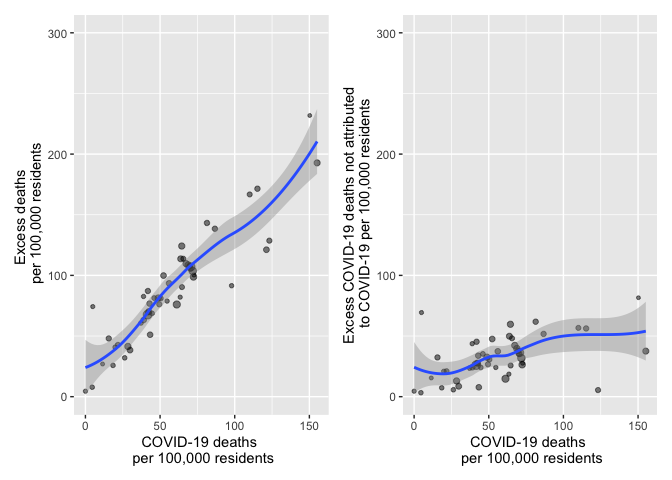
\includegraphics{analysis_files/figure-latex/unnamed-chunk-7-1.pdf}

We explore whether the duration of stay at home orders are associated
with excess non-covid related mortality. We import and link data on the
lengths of each states stay-at-home-orders based on information
aggregated from by the National Academy of State Health Policy
(\url{https://www.nashp.org/governors-prioritize-health-for-all/}). We
join these data to our state level data set plot stay-at-home order
duratoin vs non-covid-19 excess mortality rates.

\begin{Shaded}
\begin{Highlighting}[]
\NormalTok{stay_at_home_orders <-}\StringTok{ }\KeywordTok{read_csv}\NormalTok{(}\StringTok{"data/stay_at_home_orders_final.csv"}\NormalTok{, }
    \DataTypeTok{col_types =} \KeywordTok{cols}\NormalTok{(}\DataTypeTok{Start =} \KeywordTok{col_date}\NormalTok{(}\DataTypeTok{format =} \StringTok{"%m/%d/%Y"}\NormalTok{), }
        \DataTypeTok{End =} \KeywordTok{col_date}\NormalTok{(}\DataTypeTok{format =} \StringTok{"%m/%d/%Y"}\NormalTok{))) }\OperatorTok\StringTok{ }
\StringTok{  }\KeywordTok{clean_names}\NormalTok{() }\OperatorTok\StringTok{ }
\StringTok{  }\KeywordTok{mutate}\NormalTok{(}\DataTypeTok{stay_at_home=}\KeywordTok{if_else}\NormalTok{(length}\OperatorTok{==}\DecValTok{0}\NormalTok{,}\OtherTok{FALSE}\NormalTok{,}\OtherTok{TRUE}\NormalTok{))}

\NormalTok{states=}\KeywordTok{right_join}\NormalTok{(states,stay_at_home_orders)}
\end{Highlighting}
\end{Shaded}

\begin{verbatim}
## Joining, by = "state"
\end{verbatim}

\begin{Shaded}
\begin{Highlighting}[]
\NormalTok{states }\OperatorTok\StringTok{ }
\StringTok{ }\KeywordTok{ggplot}\NormalTok{( }\KeywordTok{aes}\NormalTok{(}\DataTypeTok{x=}\NormalTok{length,}\DataTypeTok{y=}\NormalTok{excess_not_covid_r, }\DataTypeTok{size=}\NormalTok{population))}\OperatorTok{+}
\StringTok{   }\KeywordTok{labs}\NormalTok{(}\DataTypeTok{x =} \StringTok{"Length of stay-at-home order (days)"}\NormalTok{, }\DataTypeTok{y =} \StringTok{"Excess COVID-19 deaths not attributed}\CharTok{\textbackslash{}n}\StringTok{ to COVID-19 per 100,000 residents"}\NormalTok{) }\OperatorTok{+}
\StringTok{   }\KeywordTok{geom_point}\NormalTok{(}\DataTypeTok{alpha=}\FloatTok{0.5}\NormalTok{)}\OperatorTok{+}
\StringTok{  }\KeywordTok{geom_smooth}\NormalTok{(, }\DataTypeTok{weight=}\StringTok{"population"}\NormalTok{)}\OperatorTok{+}
\StringTok{ }\KeywordTok{theme}\NormalTok{(}\DataTypeTok{legend.position =} \StringTok{"none"}\NormalTok{) }\OperatorTok{+}
\StringTok{  }\KeywordTok{scale_y_continuous}\NormalTok{(}\DataTypeTok{limits=}\KeywordTok{c}\NormalTok{(}\DecValTok{0}\NormalTok{, }\DecValTok{100}\NormalTok{))}
\end{Highlighting}
\end{Shaded}

\begin{verbatim}
## `geom_smooth()` using method = 'loess' and formula 'y ~ x'
\end{verbatim}

\begin{verbatim}
## Warning: Removed 2 rows containing non-finite values (stat_smooth).
\end{verbatim}

\begin{verbatim}
## Warning: Removed 2 rows containing missing values (geom_point).
\end{verbatim}

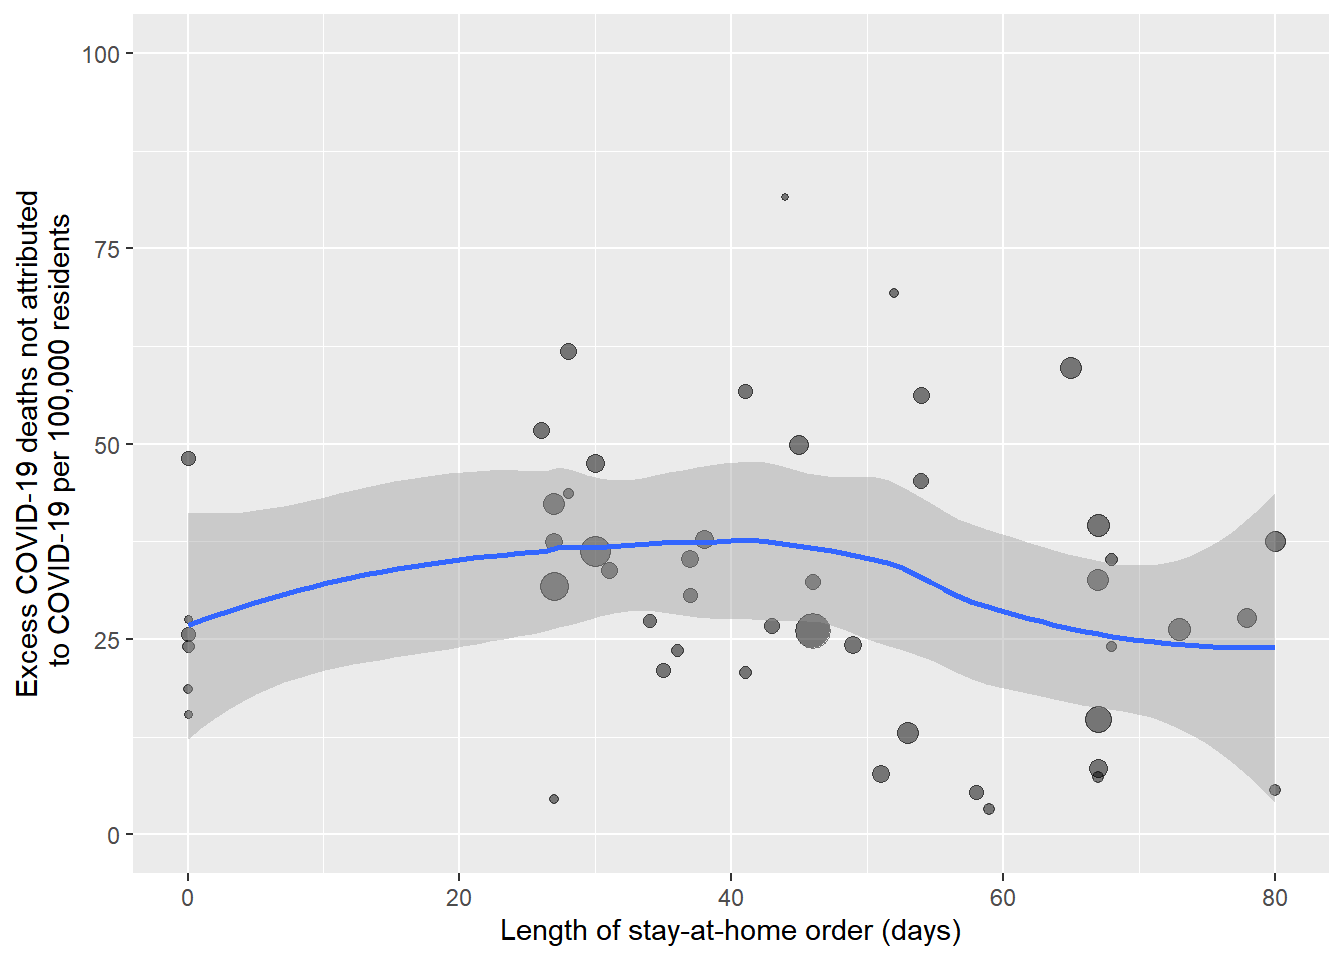
\includegraphics{analysis_files/figure-latex/unnamed-chunk-8-1.pdf}

Finally we fit some regression models to evaluate several hypothesis.

First we evaluate the hypothesis (which is pretty obvious) that state
excess mortality rate during the COVID epidemic is associated with
COVID-19 mortality. We fit a bivariable linear regression model, with
cluster robust standard errors.

\begin{Shaded}
\begin{Highlighting}[]
\KeywordTok{library}\NormalTok{(miceadds)}
\NormalTok{mod1 <-}\StringTok{ }\KeywordTok{lm.cluster}\NormalTok{(excess_death_r }\OperatorTok{~}\StringTok{ }\NormalTok{covid_death_r, }\DataTypeTok{data =}\NormalTok{ states, }\DataTypeTok{cluster=}\StringTok{"state"}\NormalTok{)}
\KeywordTok{summary}\NormalTok{(mod1) }
\end{Highlighting}
\end{Shaded}

\begin{verbatim}
## R^2= 0.84055 
## 
##                Estimate Std. Error   t value     Pr(>|t|)
## (Intercept)   20.490304  5.8769983  3.486525 4.893389e-04
## covid_death_r  1.174205  0.1071758 10.955872 6.227541e-28
\end{verbatim}

\begin{Shaded}
\begin{Highlighting}[]
\KeywordTok{confint}\NormalTok{(mod1) }
\end{Highlighting}
\end{Shaded}

\begin{verbatim}
##                   2.5 %    97.5 %
## (Intercept)   8.9715989 32.009009
## covid_death_r 0.9641438  1.384265
\end{verbatim}

Accounting for state-level clustering, we found a statistically
significant association between the COVID-19 death rate and the excess
mortality rate among US states (p\textless0.001). Each additional death
per 100,000 residents was associated was 1.2 excess deaths per 100,000
individuals (95\% CI 0.9 to 1.4). We observed that 84\% in the
variability in excess mortality among states was explained by the
COVID-19 death rate.

Next we evaluated the less obvious hypothesis that the rate of excess
death not attributable to COVID-19 was associated with the COVID-19
death rate. We fit a similar model:

\begin{Shaded}
\begin{Highlighting}[]
\NormalTok{mod2 <-}\StringTok{ }\KeywordTok{lm.cluster}\NormalTok{(excess_not_covid_r }\OperatorTok{~}\StringTok{ }\NormalTok{covid_death_r, }\DataTypeTok{data =}\NormalTok{ states, }\DataTypeTok{cluster=}\StringTok{"state"}\NormalTok{)}
\KeywordTok{summary}\NormalTok{(mod2) }
\end{Highlighting}
\end{Shaded}

\begin{verbatim}
## R^2= 0.10396 
## 
##                 Estimate Std. Error  t value     Pr(>|t|)
## (Intercept)   20.4903038  5.8769983 3.486525 0.0004893389
## covid_death_r  0.1742046  0.1071758 1.625409 0.1040753359
\end{verbatim}

\begin{Shaded}
\begin{Highlighting}[]
\KeywordTok{confint}\NormalTok{(mod2) }
\end{Highlighting}
\end{Shaded}

\begin{verbatim}
##                     2.5 %     97.5 %
## (Intercept)    8.97159886 32.0090088
## covid_death_r -0.03585615  0.3842653
\end{verbatim}

There was no statistically significant association between the rate of
excess deaths not attributed to COVID-19 and the rate of COVID-19
mortality (p=0.10).

Finally we fit a linear model (which accounts for clustering at the
state level), to tests the hypothesis that the duration of a states lock
down is associated with excess mortality to attributed to COVID=19.

\begin{Shaded}
\begin{Highlighting}[]
\KeywordTok{library}\NormalTok{(miceadds)}
\NormalTok{mod3 <-}\StringTok{ }\KeywordTok{lm.cluster}\NormalTok{(excess_not_covid_r }\OperatorTok{~}\StringTok{ }\NormalTok{length, }\DataTypeTok{data =}\NormalTok{ states, }\DataTypeTok{cluster=}\StringTok{"state"}\NormalTok{)}
\KeywordTok{summary}\NormalTok{(mod3)}
\end{Highlighting}
\end{Shaded}

\begin{verbatim}
## R^2= 0.01246 
## 
##               Estimate Std. Error    t value     Pr(>|t|)
## (Intercept) 34.5792313  4.4984495  7.6869223 1.507166e-14
## length      -0.0946756  0.0965685 -0.9803984 3.268895e-01
\end{verbatim}

\begin{Shaded}
\begin{Highlighting}[]
\KeywordTok{confint}\NormalTok{(mod3) }
\end{Highlighting}
\end{Shaded}

\begin{verbatim}
##                  2.5 %      97.5 %
## (Intercept) 25.7624324 43.39603024
## length      -0.2839464  0.09459518
\end{verbatim}

Modeling lockdown duration as a continuous variable with a linear
relationship with excess mortality, We found no statistically
significant relationship between length of lock down and excess deaths
not attributed to COVID-19 (p=0.33)

We fit another model modeling lock downs as a present/absent variable

\begin{Shaded}
\begin{Highlighting}[]
\NormalTok{mod4 <-}\StringTok{ }\KeywordTok{lm.cluster}\NormalTok{(excess_not_covid_r }\OperatorTok{~}\StringTok{ }\NormalTok{stay_at_home, }\DataTypeTok{data =}\NormalTok{ states, }\DataTypeTok{cluster=}\StringTok{"state"}\NormalTok{)}
\KeywordTok{summary}\NormalTok{(mod4)}
\end{Highlighting}
\end{Shaded}

\begin{verbatim}
## R^2= 0.00607 
## 
##                   Estimate Std. Error   t value     Pr(>|t|)
## (Intercept)      26.589738   4.370597 6.0837768 1.173840e-09
## stay_at_homeTRUE  4.474564   5.261647 0.8504113 3.950964e-01
\end{verbatim}

\begin{Shaded}
\begin{Highlighting}[]
\KeywordTok{confint}\NormalTok{(mod4) }
\end{Highlighting}
\end{Shaded}

\begin{verbatim}
##                      2.5 %   97.5 %
## (Intercept)      18.023525 35.15595
## stay_at_homeTRUE -5.838074 14.78720
\end{verbatim}

Again, while states with lockdowns had a rates of excess deaths that
were not attributed to COVID-19 that were higher by 4.5 per 100,000
residents (95\% CI -5.8 to 14.8), this association was not statistically
significant (p=0.40).

\end{document}
